\documentclass{ucetd}
\usepackage{subfigure,epsfig,amsfonts}
\usepackage{natbib}
\usepackage{amsmath}
\usepackage{amssymb}
\usepackage{amsthm}
\graphicspath{ {figures/ch3/} }
\begin{document}

\chapter{Effectors downstream of RhoA regulate pulse size and spatial dynamics}

\section{Abstract}
We have previously shown that pulsatile RhoA dynamics drive the initiation and termination of pulsed contractions in the early \textit{C.elegans} embryo.  We have shown that autocatalytic activation of RhoA precedes the assembly of F-actin, and activation of Myosin II, within pulsed contractions.  Inhibition of active RhoA, which is mediated by the redundant RhoA GAPs RGA-3 and RGA-4, precedes the disappearance of F-actin and Myosin II.  Although we understand many details about how pulsed contractions are regulated temporally, it is still unclear how pulses of active RhoA are regulated spatially.  The purpose of this chapter is to report some interesting observations that suggest that tuning effectors downstream of active RhoA plays a role in regulating spatial features of RhoA pulses such as size, lifetime, and the propensity to form traveling waves.


\section{Introduction}
Local activation of RhoA has been shown to be an important component of pulsed contractions during apical constriction during both mesoderm invagination and germ band extension in \textit{Drosophila} \cite{Mason:2013ee, Munjal:2015bx, Mason:2016bs}.  In \textit{C.elegans} embryos, autocatalytic activation of RhoA is thought to drive the accumulation of downstream factors such as F-actin, myosin II, and anillin during pulsed contractions (Figure 2.4, Figure 2.6).  RhoA promotes actin polymerization and myosin II activation through the activities of the formin CYK-1 and Rho kinase (LET-502), respectively (Figure 3.1).  Although it is unlikely that these downstream factors participate in a positive feedback with RhoA, it remains unclear how they might otherwise affect the spatial regulation of RhoA and contractile dynamics during pulsed contractions.  For example, RhoA continued to pulse in the absence of myosin II.  However, the \textit{nmy-2} RNAi pulses were qualitatively very different that wild-type pulses.  This observation raises the possibility that RhoA pulse dynamics are somehow linked to underlying actomyosin cytoskeleton.  Here, we have demonstrated that tuning effectors downstream of RhoA such as CYK-1, LET-502, and ANI-1 can affect RhoA spatial and temporal dynamics.  The purpose of this chapter is to describe and highlight these interesting phenotypes in order to provide an avenue for future research.
%Figure 3.1
\begin{figure}[!htbp]
\centering
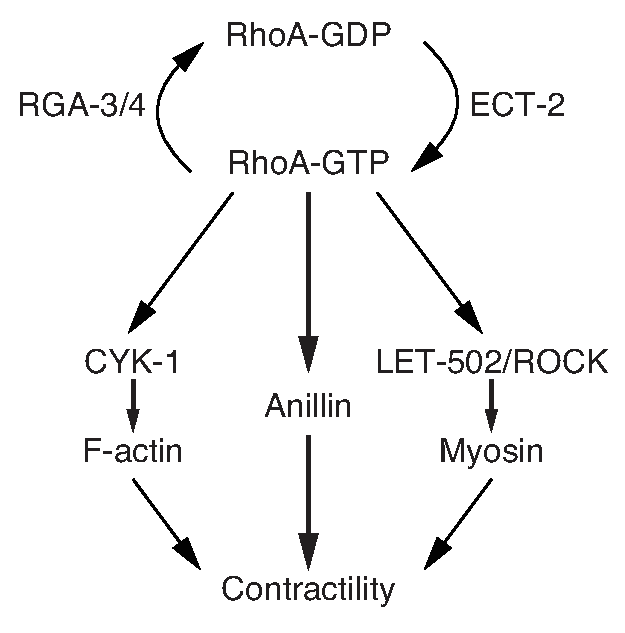
\includegraphics[width=0.45\textwidth]{Figure3-1}
\captionof{figure}[Excitable activation of RhoA drives pulsed contractility through its downstream effectors.]{\textbf{Excitable activation of RhoA drives pulsed contractility through its downstream effectors.} Local activation and deactivation of RhoA during pulsed contractions is regulated by the GEF ECT-2 and the Rho GAPs RGA-3/4, respectively. Active RhoA promotes actin polymerization through the activity of the formin CYK-1, and Myosin II activation through LET-502/ROCK.  The scaffold protein Anillin is thought to regulate pulsed contractions by stabilizing Myosin II. }
\end{figure}


\section{Results}
\subsection{RhoA does not pulse in the absence of an intact F-actin network}
Recent work from Bement \textit{et al.} has demonstrated that F-actin plays a role in negatively regulating excitable RhoA dynamics \cite{Bement:2015jp}.  In addition to playing a role as a scaffold, we hypothesize that F-actin facilitates negative feedback onto RhoA by recruiting the RhoA GAPs RGA-3 and RGA-4 during pulsed contractions in \textit{C.elegans}.  We have shown that RhoA does not pulse in the absence of RGA-3/4, but instead localizes uniformly to the cortex.  We have also shown that GFP::RGA-3 strongly co-localizes with mCherry::LifeAct on actin filaments in both P0 and AB.  Furthermore, we observed that RGA-3 does not localize to the cortex when embryos are treated with latrunculin A.  Therefore, we hypothesize that RhoA will uniformly localize to the cortex in the absence of an intact F-actin network.



To further test the idea that F-actin acts as a scaffold to promote negative feedback onto RhoA, we used latrunculin A to inhibit F-actin assembly in single-cell embryos.  Embryos were permeabilized by \textit{perm-1} RNAi and treated with 10$\mu$M latrunculin A \cite{Carvalho:2011ce}.  First, we tested whether myosin II or anillin continued to accumulate within pulses in the absence F-actin.  Upon latrunculin A treatment, we observed that GFP::ANI-1 and NMY-2::RFP did not pulse, but instead formed clusters in the absence of F-actin (Figure 3.2, top row).  Similarly, GFP::AHPH co-clustered with NMY-2::RFP in the absence of F-actin (Figure 3.2, bottom row).  These clusters were very stable, lasting the entire duration of polarity establishment (data not shown).  The clusters we observed are reminiscent of those observed by Hickson \textit{et al.} in \textit{Drosophila} S2 cells \cite{Hickson:2008hu}.  Hickson \textit{et al.} showed that anillin, myosin II, and septin all co-cluster when \textit{Drosophila} S2 cells are treated with latrunculin A during cytokinesis \cite{Hickson:2008hu}.  They also showed that the formation of these clusters was RhoA dependent and required the presence of anillin or septin \cite{Hickson:2008hu}.  These results reinforce the idea that an intact F-actin network is required for the proper recruitment of factors downstream of RhoA.

%Figure 3.2
\begin{figure}[!htbp]
\centering
\includegraphics[width=0.85\textwidth]{Figure3-2}
\captionof{figure}[Depolymerization of F-actin induces co-clustering of Myosin II, Anillin, and the active RhoA biosensor.]{\textbf{Depolymerization of F-actin induces co-clustering of Myosin II, Anillin, and the active RhoA biosensor.} Embryos co-expressing GFP::ANI-1 and NMY-2::RFP (top row) and embryos co-expressing GFP::AHPH and NMY-2::RFP (bottom row) were permeabilized by \textit{perm-1} RNAi treatment.  The addition of 10$\mu$M latrunculin A caused a complete loss of cortical F-actin and the formation of ectopic clusters containing Anillin, Myosin II, and the probe for active RhoA.}
\end{figure}

The above results suggest that RhoA does not pulse in the absence of F-actin.  However, it is possible that the RhoA biosensor accumulating within punctae is an artifact due to its ability to bind other factors through its PH domain.  To get around this, we attempted to inhibit the formation of these punctae by depolymerizing the actin cortex in a strain expressing the RhoA biosensor in a septin (UNC-59 in \textit{C.elegans}) mutant background.  In this experiment, we imaged embryos expressing GFP::AHPH before and after an acute latrunculin A treatment.  Prior to treatment, RhoA formed robust pulses on the cortex in both control and mutant embryos.  As expected, we observed the RhoA biosensor accumulate in stable punctae in control embryos in less than one minute after latrunculin A treatment (Figure 3.3, top row).  In contrast, the RhoA biosensor localized uniformly to the cortex in \textit{unc-59} mutant embryos (Figure 3.3, bottom row).  Therefore, RhoA pulses requires an intact F-actin network.
%Figure 3.3
\begin{figure}[!htbp]
\centering
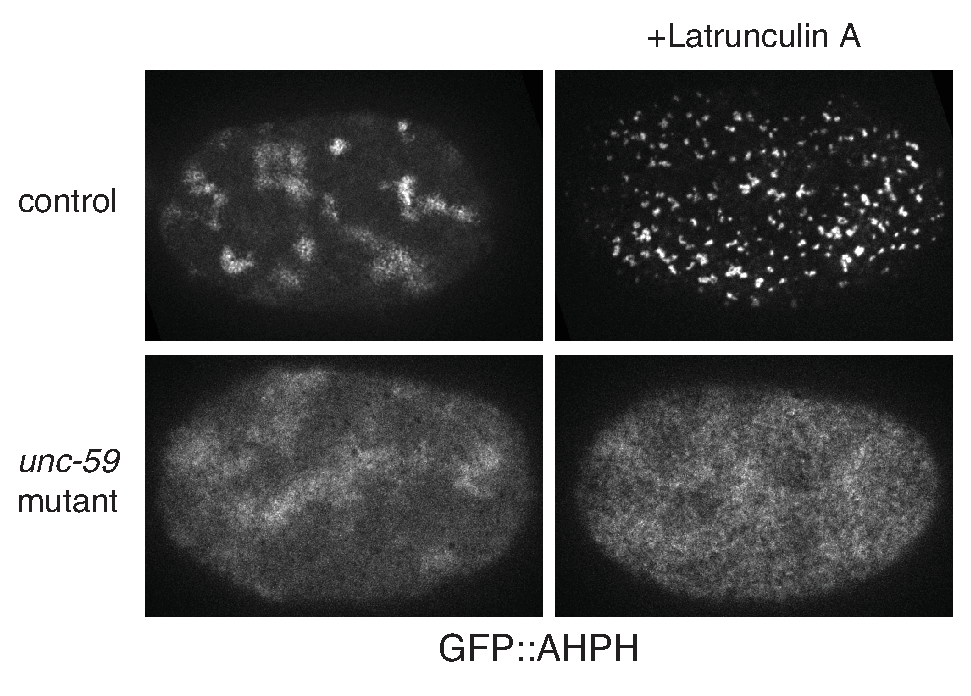
\includegraphics[width=0.65\textwidth]{Figure3-3}
\captionof{figure}[Septin mediates clustering of the active RhoA biosensor in latrunculin A treated embryos.]{\textbf{Septin mediates clustering of the active RhoA biosensor in latrunculin A treated embryos.]} Control and \textit{unc-59} mutant embryos expressing GFP::AHPH were acutely treated with 10$\mu$M latrunculin A.  In control embryos, the active RhoA biosensor formed clusters that contained Anillin and Myosin II (Figure 3.2).  In mutant embryos, active RhoA did not form clusters, but instead localized uniformly on the cortex.}
\end{figure}

\subsection{Depletion of CYK-1 affects RhoA pulse size, duration, and spatial distribution}

%cyk-1
Our previous experiments have robustly demonstrated that pulsatile RhoA activity drives pulsed contractions in \textit{C.elegans}, and that RhoA pulses do not rely on the presence of myosin II or myosin II-dependent contractility.  The fact that active RhoA does not locally pulse in the absence of F-actin, but instead localizes uniformly to the cortex, suggests that actomyosin dynamics might play role in shaping RhoA pulses.  To test this idea, we've used RNAi to mildly deplete key effectors downstream of active RhoA.  In order to compare the different phenotypes, we tracked the GFP::AHPH signal for multiple pulses, and aligned their normalized intensities relative to the time point at which GFP::AHPH reaches 25$\%$ its maximum intensity (Figure 3.5).  We also present kymographs to compare RhoA spatial dynamics.


First, we targeted the major \textit{C.elegans} formin CYK-1 \cite{Swan:1998tv}.  CYK-1, together with profilin (PFN-1 in \textit{C.elegans}) was shown to mediate the polymerization of actin filaments independent of the ARP-2/3 complex \cite{Severson:2002ve}.  Severson \textit{et al.} also showed that CYK-1 mediated actin polymerization is necessary for A-P polarity establishment as well as cytokinesis in the early embryo.  We imaged embryos co-expressing GFP::AHPH and NMY-2::RFP under conditions in which the formin CYK-1 was mildly depleted by RNAi.  RhoA and myosin II strongly co-localized within punctae within pulsed contractions as well as other regions of the cortex.  The averaged intensity profile shows that RhoA accumulates with similar kinetics in \textit{cyk-1} depleted embryos compared to wild-type embryos (Figure 3.5A).  In contrast, the duration of \textit{cyk-1} RNAi pulses appears shorter than wild-type P0 pulses (Figure 3.5A).
%Figure 3.4
\begin{figure}[!htbp]
\centering
\includegraphics[width=0.95\textwidth]{Figure3-4}
\captionof{figure}[Depletion of RhoA effectors changes RhoA spatial dynamics.]{\textbf{Depletion of RhoA effectors changes RhoA spatial dynamics.} Micrographs of single-cell P0 embryos co-expressing GFP::AHPH (top panels) and NMY-2::RFP (middle panels) under various conditions.  Pulses in \textit{cyk-1}, \textit{let-502}, and \textit{ani-1} RNAi embryos appeared larger than pulses in wild-type embryos.  (Bottom panels) The dashed yellow box indicates the region of each micrograph in the top panels used to make the kymograph.  The kymographs reveal a decrease in cortical flow in \textit{cyk-1}, \textit{let-502}, and \textit{ani-1} RNAi embryos compared to wild-type embryos.  Pulses in \textit{cyk-1} and \textit{ani-1} RNAi embryos appear to have a shorter duration than wild-type and \textit{let-502} embryos.}
\end{figure}

We also observed that RhoA pulses appeared spatially larger in \textit{cyk-1} depleted embryos than in wild-type embryos (Figure 3.4, first and second  columns).  We quantified this by measuring the ratio of the size of RhoA pulses relative to the size of the embryo in which they were observed (Figure 3.5B).  On average, \textit{cyk-1} RNAi pulses were about 6$\%$ the size of the embryo, while wild-type pulses were about 2.5$\%$ the size of the embryo.  A visual inspection of \textit{cyk-1} depleted embryos suggests that fewer RhoA pulses form on the cortex an any given time.  A comparison of kymographs from representative wild-type and \textit{cyk-1} depleted embryos shows a decrease in cortical flow in \textit{cyk-1} embryos during polarity establishment.  These data suggest that CYK-1-mediated actin assembly plays a role in regulating RhoA spatial dynamics.

\subsection{Depletion of LET-502 affects RhoA pulse size and spatial dynamics}
%let-502
Our previous results support the idea that RhoA pulses are independent of myosin II (see Chapter 2).  However, in the absence of myosin II RhoA pulses were qualitatively and quantitatively different than pulses in wild-type pulses.  The \textit{nmy-2} RNAi pulses appeared weaker, and also shorter than wild-type pulses.  Munjal \textit{et al.} showed that inhibiting Rho kinase (Rok in \textit{Drosophila}, LET-502 in \textit{C.elegans}) with the inhibitor Y27632 abolished RhoA pulses, as well as blocked the cortical recruitment of other factors involved in pulsed contractions during germband extension \cite{Munjal:2015bx}.  Therefore, we wondered if depleting LET-502 would weaken RhoA pulses or completely eliminate them.  As expected, there was a marked decrease in myosin II both on the cortex and within pulsed contractions (Figure 3.4, third column).  We also observed a decrease in cortical flow during polarity establishment (Figure 3.4, third column).  These results are consistent with LET-502 being a key activator of myosin II activity.  Surprisingly, however,  RhoA continued to pulse robustly under strong \textit{let-502} RNAi conditions (Figure 3.4, third column).  Similar to \textit{cyk-1} RNAi pulses, \textit{let-502} RNAi pulses were also larger than wild-type P0 pulses (Figure 3.5B).  Furthermore, \textit{let-502} RNAi pulses showed an increased propensity for forming traveling waves.  Although \textit{let-502} RNAi pulses exhibited different spatial dynamics than wild-type pulses, the initiation and termination kinetics appear similar to wild-type P0 pulses.  Therefore, strong depletion of LET-502 does not inhibit RhoA pulses, but instead alters RhoA pulse size and spatial dynamics.




\subsection{Depletion of ANI-1 affects RhoA pulse size and duration}
%ani-1
Anillin (ANI-1 in \textit{C.elegans}) is a scaffold protein that plays an important role in regulating actomyosin contractility during cytokinesis in human and \textit{Drosophila} cells \cite{Piekny:2010es}.  It is thought to bind F-actin, myosin II, septins, ECT-2, RhoA and other proteins \cite{Piekny:2010es}.  Maddox \textit{et al.} showed that ANI-1 plays a role in polar body extrusion, asymmetric cell division, and cortical ruffling (i.e., pulsed contractions) and pseudocleavage during polarity establishment \cite{Maddox:2005gd}.  They reported a nearly complete loss of myosin II pulses in P0 under strong \textit{ani-1} RNAi conditions \cite{Maddox:2005gd}.  Under these conditions, myosin II localizes uniformly to the cortex instead of in dense foci.  In contrast, ANI-1 patches remained on the cortex in the absence of myosin II.  The authors proposed that ANI-1-mediated positive feedback drives pulsed contractions by binding and \cite{Maddox:2005gd}.  In their model, ANI-1 is recruited locally to the cortex through its PH- and actin-binding domains, where ANI-1 then promotes its own accumulation by recruiting F-actin.

We have shown that the accumulation of RhoA within pulsed contractions is autocatalytic, and that activate RhoA precedes the accumulation of F-actin, myosin II, and anillin within pulsed contractions (see Chapter 2).  Although our results argue against anillin initiating pulsed contractions, it is still not clear how anillin might affect RhoA dynamics during pulsed contractions.  To test this, embryos expressing the active RhoA biosensor and NMY-2::RFP were depleted of ANI-1 via RNAi.  Since the biosensor is made from a fragment of ANI-1, we used RNAi targeting anillin's myosin binding domain.  The \textit{ani-1 (myo)} RNAi phenotype was characterized by a loss of pseudoclavage and a decrease in cortical flow (Figure 3.4, fourth column).  Although RhoA and myosin II still accumulated in pulses, myosin II did not form dense foci similar to pulsed contractions in wild-type embryos.  Similar to the \textit{cyk-1} RNAi phenotype, \textit{ani-1 (myo)} RNAi pulses were larger than P0 pulses (Figure 3.5B).  Furthermore, \textit{ani-1 (myo)} RNAi appeared to be shorter in duration than P0 pulses (Figure 3.5A).  Taken together, these results suggest that ANI-1 might play a role in stabilizing myosin II within pulsed contractions as well as limiting the size of RhoA pulses.

%Figure 3.5
\begin{figure}[!htbp]
\centering
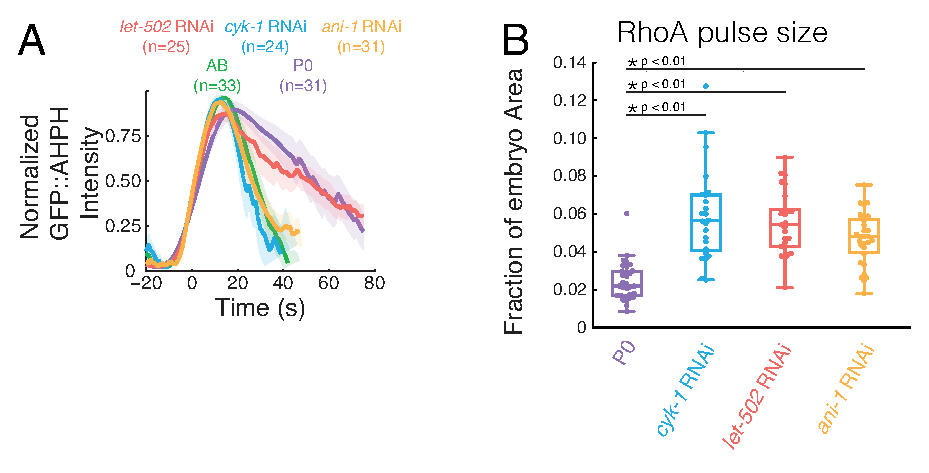
\includegraphics[width=0.85\textwidth]{Figure3-5}
\captionof{figure}[Quantification of RhoA pulse size and duration.]{\textbf{Quantification of RhoA pulse size and duration.} (A) Comparison of averaged normalized fluorescence intensities vs time for active RhoA (GFP::AHPH).  Data were co-aligned with respect to the time at which GFP::AHPH reaches 25$\%$ threshold. Hued regions report 95$\%$ confidence intervals. (B) Knocking down various RhoA effectors changes the size of RhoA pulses.  The size of each RhoA pulse was measured at the time at which GFP::AHPH fluorescence intensity reached its max.  Each measurement was normalized by the area of the embryo in which the pulse occured. }
\end{figure}


Although our results argue against the model proposed by Maddox \textit{et al.}, we have not ruled out the possibility that anillin is required for RhoA pulses.  This is largely due to the inefficiency of knocking down ANI-1 when targeting its myosin binding domain.  To get around this, we wanted to use RNAi to target full length ANI-1 in embryos co-expressing NMY-2::RFP and  fully labeled GFP::LET-502 (made by Thanh Vuong, Labouesse lab).  As a control, we compared embryos expressing GFP::LET-502 to embryos expressing GFP::AHPH.  In wild-type embryos, LET-502's distribution on the cortex is reminiscent of the RhoA biosensor (Figure 3.4 and Figure 3.6).  LET-502 also co-localizes with NMY-2::RFP within pulsed contractions (Figure 3.6, first column).   In order to confirm that the accumulation of LET-502 on the cortex is RhoA dependent, we used RNAi to partially knockdown RhoA (RHO-1 in \textit{C.elegans}).  We observed a strong decrease in cortical GFP::LET-502 during polarity establishment in \textit{rho-1} RNAi embryos (Figure 3.6, second column).  Consistent with this phenotype, partial \textit{rho-1} RNAi embryos also exhibited a decrease in cortical NMY-2::RFP and pulsed contractions (Figure 3.6, second column).  These data suggest that full-length GFP::LET-502 can be used as an alternate biosensor for detecting active RhoA on the cortex.


Thus, to determine if RhoA continues to pulse in the absence of ANI-1 we treated embryos co-expressing GFP::LET-502 and NMY-2::RFP with RNAi targeting ANI-1.  As expected, \textit{ani-1} RNAi embryos did not form a pseudocleavage furrow (Figure 3.6, third column).  We also observed a strong decrease in NMY-2::RFP pulse formation.  Interestingly, we did not observe a complete loss of myosin II pulses as reported by Maddox \textit{et al.} \cite{Maddox:2005gd}.  NMY-2::RFP did not accumulate in dense foci that correspond to deep membrane invaginations like in wild-type embryos (Figure 3.6, third column).  Instead NMY-2::RFP accumulated in transient pulses that appeared much weaker and shorter than wild-type pulses.  Our observations seem to contradict those reported by Maddox \textit{et al.}.  However, a close inspection of their supplemental movie data shows GFP::NMY-2 forming transient pulses during polarity establishment under strong \textit{ani-1} RNAi conditions \cite{Maddox:2005gd}.  We also observed that GFP::LET-502 continued to form robust pulses in the absence of ANI-1.  Control embryos co-expressing GFP::ANI-1 and NMY-2::RFP showed a drastic decrease in GFP::ANI-1 fluorescence intensity under \textit{ani-1} RNAi conditions (See Chapter 2, Figure 3.6, fourth column).  Together, these results suggest that although anillin is not required for RhoA pulses, it may play an important role in spatially regulating pulsed contractions.

%Figure 3.6
\begin{figure}[!htbp]
\centering
\includegraphics[width=0.95\textwidth]{Figure3-6}
\captionof{figure}[Rho kinase pulses in the absence of Anillin.]{\textbf{Rho kinase pulses in the absence of Anillin.} Micrographs of single-cell P0 embryos co-expressing GFP::LET-502 or GFP::ANI-1 (top panels) and NMY-2::RFP (middle panels) under various conditions.  (Bottom panels) The dashed yellow box indicates the region of each micrograph in the top panels used to make the kymograph.  (First column) wild-type GFP::LET-502 spatial dynamics are similar to the active RhoA biosensor.  (Second column) GFP::LET-502 does not accumulate on the cortex in partial \textit{rho-1} RNAi embryos. The kymograph shows cortical flows are still present in partial \textit{rho-1} RNAi embryos.  (Third column) GFP::LET-502 forms pulses under strong \textit{ani-1} RNAi conditions.  (Fourth column) Strong loss of fluorescence in control embryos co-expressing GFP::ANI-1 and NMY-2::RFP is indicative of a strong \textit{ani-1} RNAi phenotype..}
\end{figure}

\section{Discussion}
The work presented in this chapter demonstrates that RhoA pulses are not completely independent from the activity and dynamics of RhoA effector proteins.  We have shown that depolymerizing F-actin with latrunculin A completely eliminates RhoA pulsing (Figure 3.3).  Instead, RhoA localized uniformly to the cortex in the absence of F-actin.  This result recapitulates our previous result in which RhoA no longer pulses in the \textit{rga3/4} mutant background  (Figure 2.7).  Together, these results are consistent with our current working model, in which RhoA-dependent F-actin polymerization promotes the delayed accumulation of the Rho GAPs RGA-3 and RGA-4 that turns RhoA activity off (Figure 2.9).

The fact that RhoA does not pulse in the absence of an intact F-actin network raises the possibility that tuning the concentration of various regulators of the actomyosin cytoskeleton might alter RhoA dynamics in space or time.  We have shown that mild depletion of the formin CYK-1 disrupts RhoA spatial patterning, as well as causes RhoA pulses to become larger spatially, and shorter temporally.  Surprisingly, we also observed an increase in RhoA pulse size following the depletion Rho kinase.  In addition, we observed that RhoA pulses have a tendency to form traveling waves when Rho kinase is depleted.  This is in contrast to \textit{nmy-2} RNAi pulses, which appeared to oscillate and have a size similar to wild-type pulses.  These observations suggest that Rho kinase regulates RhoA dynamics independent of myosin II.  For example, it is possible that direct interactions between RhoA and Rho kinase prevent RhoA from spreading to nearby regions of the cortex.  Lastly, we observed a decrease in the lifetime of RhoA and myosin II pulses in the absence of anillin, even though LET-502 continued to form pulses on the cortex.  This suggest that anillin plays a role in recruiting and/or stabilizing myosin II on the cortex.  Taken together, the results presented in this chapter suggest that RhoA pulses are an emergent phenomenon, and their dynamics rely heavily on the structure and dynamics of the underlying actomyosin cytoskeleton.  Although the mechanism for generating RhoA pulses is still unclear, we believe that the phenotypes presented here will provide exciting avenues for future experiments (see Chapter 4).


\section{Materials and Methods}
For information about \textit{C.elegans} culture and strains, microscopy, pulse tracking and analysis, and kymograph analysis please refer to the materials and methods section of Chapter 2.

\subsection{RNA Interference}
RNA interference was performed by a well established feeding method \cite{Timmons:2001wg}.  Bacteria targeting \textit{spd-5}, \textit{perm-1}, \textit{ani-1} (Full length), \textit{rho-1}, \textit{let-502}, \textit{cyk-1} were obtained from the Kamath feeding library \cite{Kamath:2003bk}.  The \textit{ani-1} (myo) RNAi feeding strain that targets Anillin's myosin binding domain was a kind gift from the Glotzer lab.  For the experiments involving \textit{spd-5}, L4 larvae were transferred to \textit{spd-5} RNAi feeding plates for 24-30 hours before imaging.  For the latrunculin A experiments, late-stage L4 larvae were transfered to \textit{perm-1} RNAi feeding plates for 12-16 hours before imaging.  For the Anillin RNAi experiments, late-stage L4 larvae were transferred to \textit{ani-1} (full length) or \textit{ani-1} (myo) RNAI feeding plates for \(>\)  30 hours.  In the \textit{ani-1} (full length) experiments, A strong phenotype was verified in embryos co-expressing GFP::ANI-1 and NMY-2::RFP as a strong loss of GFP fluorescence, loss of pseudocleavage furrow formation, and the presence of transient NMY-2::RFP pulses.  The loss of pseudocleavage and the pattern of transient NMY-2::RFP pulses was used to assess the strength of the \textit{ani-1} phenotype in embryos co-expressing GFP::LET-502 and NMY-2::RFP.  For the RhoA experiments, young adults were transferred to \textit{rho-1} RNAi feeding plates 10-16 hours before imaging.  For experiments involving \textit{let-502} or \textit{cyk-1} RNAi, late-stage L4 larvae were transferred to feeding plates 24-30 hours before imaging.

\subsection{RhoA pulse size analysis}

RhoA (GFP::AHPH) pulses from  were detected, tracked, and analyzed as described in Chapter 2.  In order to measure the size of a RhoA pulse, we first extracted the size of the binary mask at the time RhoA reached its peak intensity.  We then segmented (by hand) the embryo that each pulse originated from and created a binary mask.  The area of the pulse mask and embryo mask were computed using built in MATLAB functions.  The pulse areas reported in the text and Figure 3.5 represent the ratio between the area of the pulse mask to the area of the embryo mask.


\end{document}
